%%%%%%%%%%%%%%%%%%%%%%%%%%%%%%%%%%%%%%%%%%%%%%%%%%%%%%%%%%%%%%%%%%%%%%%%

%%% LaTeX Template for ECAI Papers
%%% Prepared by Ulle Endriss (version 1.0 of 2023-12-10)

%%% To be used with the ECAI class file ecai.cls.
%%% You also will need a bibliography file (such as mybibfile.bib).

%%%%%%%%%%%%%%%%%%%%%%%%%%%%%%%%%%%%%%%%%%%%%%%%%%%%%%%%%%%%%%%%%%%%%%%%

%%% Start your document with the \documentclass{} command.
%%% Use the first variant for the camera-ready paper.
%%% Use the second variant for submission (for double-blind reviewing).

\documentclass{ecai}
%\documentclass[doubleblind]{ecai}

%%%%%%%%%%%%%%%%%%%%%%%%%%%%%%%%%%%%%%%%%%%%%%%%%%%%%%%%%%%%%%%%%%%%%%%%

%%% Load any packages you require here.

\usepackage{latexsym}
\usepackage{amssymb}
\usepackage{amsmath}
\usepackage{amsthm}
\usepackage{booktabs}
\usepackage{enumitem}
\usepackage{graphicx}
\usepackage{color}
\usepackage{tikz}
\usetikzlibrary{shapes.geometric, arrows.meta, positioning, fit,
                backgrounds, decorations.pathreplacing, calc}

% ── Colour palette ────────────────────────────────────────────────────────────
\definecolor{localcol}{HTML}{2E86AB}   % steel blue  – local/private
\definecolor{cloudcol}{HTML}{E87722}   % amber       – cloud
\definecolor{kgcol}{HTML}{4C956C}      % green       – knowledge graph
\definecolor{agentcol}{HTML}{6A4C93}   % purple      – agent
\definecolor{conncol}{HTML}{C77DFF}    % lavender    – connectors
\definecolor{monoccol}{HTML}{F4A261}   % warm orange – monitor
\definecolor{headercol}{HTML}{1A1A2E}  % near-black  – headers

%%%%%%%%%%%%%%%%%%%%%%%%%%%%%%%%%%%%%%%%%%%%%%%%%%%%%%%%%%%%%%%%%%%%%%%%

%%% Define any theorem-like environments you require here.

\newtheorem{theorem}{Theorem}
\newtheorem{lemma}[theorem]{Lemma}
\newtheorem{corollary}[theorem]{Corollary}
\newtheorem{proposition}[theorem]{Proposition}
\newtheorem{fact}[theorem]{Fact}
\newtheorem{definition}{Definition}

%%%%%%%%%%%%%%%%%%%%%%%%%%%%%%%%%%%%%%%%%%%%%%%%%%%%%%%%%%%%%%%%%%%%%%%%

%%% Define any new commands you require here.

\newcommand{\BibTeX}{B\kern-.05em{\sc i\kern-.025em b}\kern-.08em\TeX}
\newcommand{\km}{\textsc{KnowledgeMind}}

%%%%%%%%%%%%%%%%%%%%%%%%%%%%%%%%%%%%%%%%%%%%%%%%%%%%%%%%%%%%%%%%%%%%%%%%

\begin{document}

%%%%%%%%%%%%%%%%%%%%%%%%%%%%%%%%%%%%%%%%%%%%%%%%%%%%%%%%%%%%%%%%%%%%%%%%

\begin{frontmatter}

%%% Use this command to specify your submission number.
%%% In doubleblind mode, it will be printed on the first page.

\paperid{1}

%%% Use this command to specify the title of your paper.

\title{KnowledgeMind: A Privacy-Aware Personal AI Agent with an
On-Device Knowledge Graph and Hybrid Local/Cloud Routing}

%%% Authors. This work was carried out as a course project for the
%%% Deep Learning course taught by Prof. Deepak Subramani at IISc Bengaluru.
%%% TODO: confirm your name spelling, add co-authors if any, and your ORCID.

% \author[A]{\fnms{Aarif}~\snm{Zafar}\thanks{Corresponding Author. Email: aarifzafar@iisc.ac.in. This work was carried out as a course project for the Deep Learning course taught by Prof.~Deepak Subramani.}}
\author[A]{\fnms{Aarif}~\snm{Z.}\footnote{Equal contribution.}}
\author[A]{\fnms{Sourav}~\snm{T.}\footnotemark}
\author[A]{\fnms{Sathyanarayanan}~\snm{K.}\footnotemark}
\author[A]{\fnms{Sarthak}~\snm{S.}\footnotemark}
\author[A]{\fnms{Novoneel}~\snm{C.}\footnotemark}
\author[A]{\fnms{Rakshit}~\snm{R.}\footnotemark}
\author[A]{\fnms{Swarup}~\snm{E.}\footnotemark}

\address[A]{Indian Institute of Science, Bengaluru, India}

%%% Use this environment to include an abstract of your paper.

\begin{abstract}
% TODO: tighten once the evaluation numbers are final (keep under 200 words).
Personal AI assistants often require access to a user's most sensitive
data, such as their calendar, messages, and email, yet most route that data to
remote large language models. We present \km, a privacy-aware personal agent
that runs entirely on commodity hardware (CPU-only) and treats on-device
processing as a hard invariant. \km{} ingests a user's communication channels,
extracts both hard commitments (calendar events) and soft commitments (informal
agreements in chat) into a personal knowledge graph built on SQLite and
NetworkX, and proactively detects scheduling conflicts across the user's whole
timeline before they occur. A privacy router scores every task on privacy and
complexity and dispatches it to a local model (via Ollama) or, only when the
task is non-sensitive, to a free cloud model; privacy always takes precedence
over complexity. The agent supports three levels of agency, from a single
augmented call to a full ReAct loop with replanning, and falls back to mock data
when no credentials are present. We describe the architecture, the privacy contract,
and an offline evaluation of routing accuracy and conflict detection.
\end{abstract}

\end{frontmatter}

%%%%%%%%%%%%%%%%%%%%%%%%%%%%%%%%%%%%%%%%%%%%%%%%%%%%%%%%%%%%%%%%%%%%%%%%

\section{Introduction}

Personal AI assistants promise to reason over a user's calendar, messages, and
email, but doing so typically means sending that data to a remote model. \km{}
takes the opposite stance: all personal data is processed locally, and only
anonymised, non-sensitive work is ever routed to the cloud.

\noindent\textbf{Problem statement.} Given a heterogeneous stream of
communication artefacts (chat messages, calendar events, emails), the system
must (i)~extract implicit and explicit commitments from natural language,
(ii)~fuse them into a temporally consistent personal knowledge graph,
(iii)~detect and proactively surface conflicts, and (iv)~do so without
transmitting personal data beyond the user's device.

\noindent\textbf{Contributions.}
\begin{itemize}[noitemsep]
  \item A privacy-pinned hybrid router that keeps a fixed set of personal-data
        tools on the local model, with per-tool minimum privacy floors that
        resist adversarial phrasing.
  \item A dual-tier commitment-extraction pipeline combining spaCy NER with
        few-shot LLM prompting and confidence-graded output
        (\textsc{hard}\,/\,\textsc{soft}\,/\,\textsc{tentative}).
  \item A personal knowledge graph with a proactive monitor that detects temporal
        conflicts across the user's whole timeline and emits dismissable nudges
        with quiet-hour suppression.
  \item A three-level ReAct orchestrator (L1 to L3) and an integrated Project
        Advisor that together span single-shot answers to multi-step replanning.
\end{itemize}

%%%%%%%%%%%%%%%%%%%%%%%%%%%%%%%%%%%%%%%%%%%%%%%%%%%%%%%%%%%%%%%%%%%%%%%%

\section{Related work and market landscape}\label{sec:related}

\km{} sits at the intersection of three lines of work: tool-using LLM agents,
the fusion of language models with knowledge graphs, and on-device
privacy-preserving inference. Our agent loop follows the ReAct paradigm of
interleaved reasoning and acting \citep{yao2023react}, and our use of a
structured personal graph as the agent's memory follows the roadmap for unifying
LLMs with knowledge graphs \citep{pan2024kg}. The distinguishing constraint is
that all of this runs locally on a small model \citep{qwen2024}, orchestrated by
a stateful graph executor \citep{langgraph2024}.

Existing tools each cover at most one or two of five capabilities (ingestion,
extraction, memory, privacy, proactivity): calendars own confirmed events but
ignore chat; task managers such as Todoist need manual entry; and cloud
assistants such as Microsoft Copilot, ChatGPT, and Gemini summarise well but
retain no user-controlled graph and send all data off-device
\citep{ms2024copilot,openai2024gpt4,notion2024}. \km{} closes all five gaps in a
single local agent, extensible through a Model Context Protocol (MCP) server. A
full feature-by-feature comparison and per-tool discussion appear in
Appendix~\ref{app:comparison} (Table~\ref{tab:comparison}).

%%%%%%%%%%%%%%%%%%%%%%%%%%%%%%%%%%%%%%%%%%%%%%%%%%%%%%%%%%%%%%%%%%%%%%%%

\section{System overview}

\begin{figure}[h]
\centering
\resizebox{\columnwidth}{!}{%
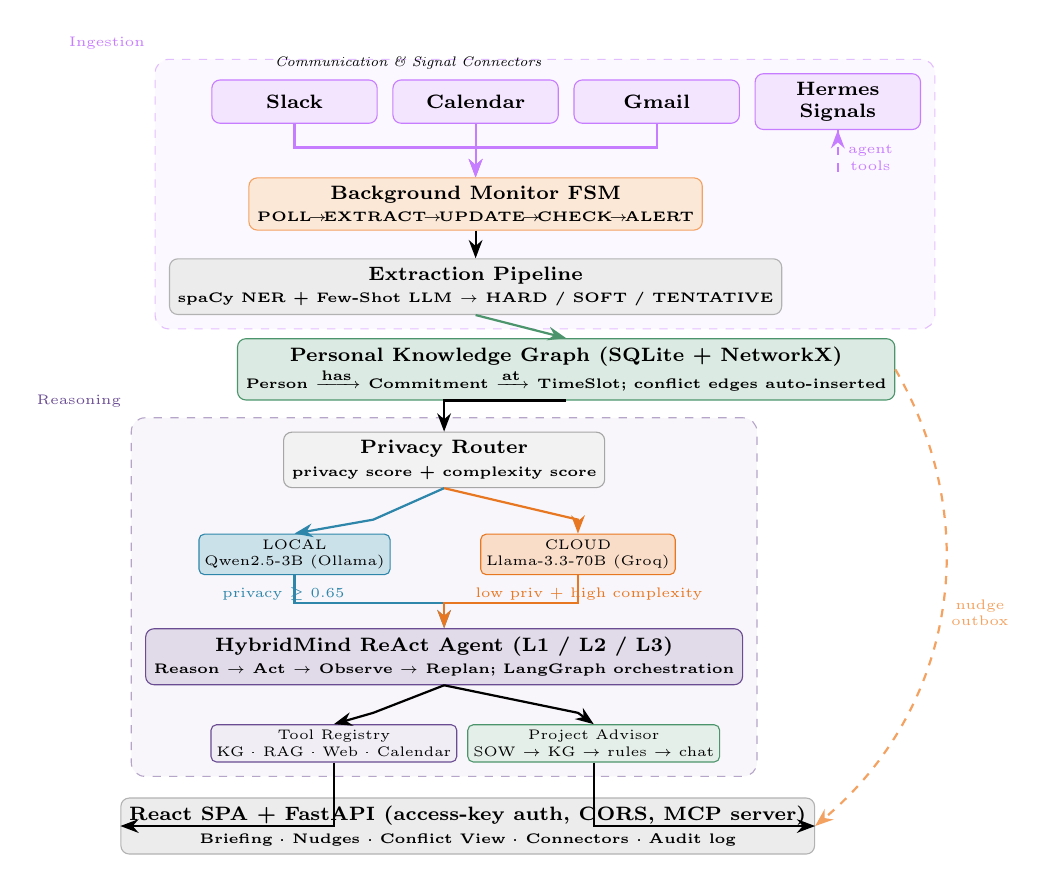
\begin{tikzpicture}[
  font=\scriptsize,
  >=Stealth,
  every node/.style={align=center},
  box/.style={draw, rounded corners=3pt, minimum width=2.1cm,
              minimum height=0.55cm, inner sep=3pt, font=\scriptsize\bfseries},
  smallbox/.style={draw, rounded corners=2pt, minimum width=1.6cm,
                   minimum height=0.45cm, inner sep=2pt, font=\tiny},
  arr/.style={->, thick},
  grp/.style={draw, dashed, rounded corners=5pt, inner sep=5pt}
]

%% ── Row 0 : Channels ──────────────────────────────────────────────────────
\node[box, fill=conncol!20, draw=conncol] (slack)   at (0,   0)    {Slack};
\node[box, fill=conncol!20, draw=conncol] (cal)     at (2.3, 0)    {Calendar};
\node[box, fill=conncol!20, draw=conncol] (gmail)   at (4.6, 0)    {Gmail};
\node[box, fill=conncol!20, draw=conncol] (hermes)  at (6.9, 0)    {Hermes\\Signals};

\node[font=\tiny, above=0pt of slack, xshift=1.45cm]
      {\textit{Communication \& Signal Connectors}};

%% ── Row 1 : Monitor FSM ───────────────────────────────────────────────────
\node[box, fill=monoccol!25, draw=monoccol,
      minimum width=5.0cm] (monitor) at (2.3, -1.3)
      {Background Monitor FSM\\{\tiny POLL$\!\to\!$EXTRACT$\!\to\!$UPDATE$\!\to\!$CHECK$\!\to\!$ALERT}};

\foreach \s in {slack, cal, gmail}
  \draw[arr, color=conncol] (\s.south) -- +(0,-0.3) -| (monitor.north);
\draw[arr, color=conncol, dashed] (hermes.south) -- +(0,-0.55)
      node[right, font=\tiny, yshift=0.2cm]{agent\\tools} +(0,0);

%% ── Row 1b : Extraction ───────────────────────────────────────────────────
\node[box, fill=gray!15, draw=gray!60,
      minimum width=4.6cm] (extract) at (2.3, -2.35)
      {Extraction Pipeline\\{\tiny spaCy NER + Few-Shot LLM $\to$ HARD / SOFT / TENTATIVE}};

\draw[arr] (monitor.south) -- (extract.north);

%% ── Row 2 : Knowledge Graph ───────────────────────────────────────────────
\node[box, fill=kgcol!20, draw=kgcol,
      minimum width=6.8cm] (kg) at (3.45, -3.4)
      {Personal Knowledge Graph (SQLite + NetworkX)\\
       {\tiny Person $\xrightarrow{\text{has}}$ Commitment $\xrightarrow{\text{at}}$ TimeSlot; conflict edges auto-inserted}};

\draw[arr, color=kgcol] (extract.south) -- (kg.north);

%% ── Row 3 : Router ────────────────────────────────────────────────────────
\node[box, fill=gray!10, draw=gray!70,
      minimum width=3.8cm] (router) at (1.9, -4.55)
      {Privacy Router\\{\tiny privacy score + complexity score}};

\draw[arr] (kg.south) -| (router.north);

%% LOCAL / CLOUD branches
\node[smallbox, fill=localcol!25, draw=localcol] (local) at (0.0, -5.75)
      {LOCAL\\{\tiny Qwen2.5-3B (Ollama)}};
\node[smallbox, fill=cloudcol!25, draw=cloudcol] (cloud) at (3.6, -5.75)
      {CLOUD\\{\tiny Llama-3.3-70B (Groq)}};

\draw[arr, color=localcol]  (router.south) -- +(-0.9,-0.4) -- (local.north);
\draw[arr, color=cloudcol]  (router.south) -- +(+1.7,-0.4) -- (cloud.north);

\node[font=\tiny, color=localcol, below=1pt of local, xshift=-4pt]
      {privacy $\geq$ 0.65};
\node[font=\tiny, color=cloudcol, below=1pt of cloud, xshift=4pt]
      {low priv + high complexity};

%% ── Row 4 : Agent ─────────────────────────────────────────────────────────
\node[box, fill=agentcol!20, draw=agentcol,
      minimum width=4.6cm] (agent) at (1.9, -7.05)
      {HybridMind ReAct Agent (L1 / L2 / L3)\\
       {\tiny Reason $\to$ Act $\to$ Observe $\to$ Replan; LangGraph orchestration}};

\draw[arr, color=localcol] (local.south) -- +(0,-0.35) -| (agent.north);
\draw[arr, color=cloudcol] (cloud.south) -- +(0,-0.35) -| (agent.north);

%% ── Row 5 : Tools + Proj Advisor ──────────────────────────────────────────
\node[smallbox, fill=agentcol!10, draw=agentcol,
      minimum width=2.7cm] (tools) at (0.5, -8.15)
      {Tool Registry\\{\tiny KG · RAG · Web · Calendar}};
\node[smallbox, fill=kgcol!15, draw=kgcol,
      minimum width=2.6cm] (pm) at (3.8, -8.15)
      {Project Advisor\\{\tiny SOW $\to$ KG $\to$ rules $\to$ chat}};

\draw[arr] (agent.south) -- +(-0.9,-0.35) -- (tools.north);
\draw[arr] (agent.south) -- +(+1.7,-0.35) -- (pm.north);

%% ── Row 6 : Interface ─────────────────────────────────────────────────────
\node[box, fill=gray!15, draw=gray!60,
      minimum width=6.2cm] (ui) at (2.2, -9.2)
      {React SPA + FastAPI (access-key auth, CORS, MCP server)\\
       {\tiny Briefing · Nudges · Conflict View · Connectors · Audit log}};

\draw[arr] (tools.south) |- (ui.west);
\draw[arr] (pm.south) |- (ui.east);

%% ── Proactive nudge feedback arc ──────────────────────────────────────────
\draw[arr, color=monoccol, dashed, bend left=40]
      (kg.east) to node[right, font=\tiny]{nudge\\outbox} (ui.east);

%% ── Group labels ──────────────────────────────────────────────────────────
\begin{scope}[on background layer]
  \node[grp, draw=conncol!50,  fill=conncol!5,
        fit=(slack)(cal)(gmail)(hermes)(monitor)(extract),
        label={[font=\tiny\color{conncol}]north west:Ingestion}] {};
  \node[grp, draw=agentcol!50, fill=agentcol!5,
        fit=(router)(local)(cloud)(agent)(tools)(pm),
        label={[font=\tiny\color{agentcol}]north west:Reasoning}] {};
\end{scope}

\end{tikzpicture}}%
\caption{KnowledgeMind system architecture.
  Blue boxes: local-only; amber: cloud-eligible; green: knowledge graph;
  purple: agent and reasoning; dashed arrows: asynchronous paths.}
\label{fig:arch}
\end{figure}

\km{} is structured as a single FastAPI backend that both serves a React
single-page application and wraps the engine. Every request is gated by an
optional access key; the application runs CPU-only and degrades to mock data
whenever a connector's credentials are absent, so the full pipeline is
exercisable offline. The engine is organised as a pipeline of six layers
(Figure~\ref{fig:arch}).

\begin{description}[leftmargin=1.2em,itemsep=2pt]
  \item[Ingestion.] Connectors for Slack, Calendar, and Gmail expose a common
        \texttt{fetch\_recent} interface and fall back to mock data on a failed
        health check. A separate family of \emph{signal} connectors (fitness,
        sleep, tasks, music) derives on-device features rather than messages.
  \item[Extraction.] A spaCy named-entity pass and a few-shot local LLM map
        raw messages into commitments, with a relative-time resolver mapping
        expressions such as ``tomorrow'' or ``EOD'' to absolute time
        (Section~\ref{sec:kg}).
  \item[Knowledge graph.] Commitments are persisted in SQLite and assembled
        into a NetworkX graph on demand; temporal conflicts are detected
        incrementally on insert (Section~\ref{sec:kg}).
  \item[Routing.] A privacy router classifies every task step as \textsc{local}
        or \textsc{cloud} before any model is called (Section~\ref{sec:routing}).
  \item[Agent.] A hybrid agent dispatches a shared registry of tools at one of
        three levels of agency, injecting only structured graph summaries before
        any cloud call (Section~\ref{sec:agent}).
  \item[Proactive layer.] A finite-state monitor fires unprompted conflict
        alerts, and an optional, off-by-default runtime composes nudges and a
        daily briefing entirely on-device (Section~\ref{sec:proactive}).
\end{description}

The central design invariant is that all personal data (graph nodes, messages,
calendar events, email bodies, and derived health or activity signals) is
processed locally at all times. The cloud model receives only anonymised
task descriptions, structured knowledge-graph summaries, and non-sensitive
public queries. The next two sections make this invariant precise and describe
how it is enforced.

%%%%%%%%%%%%%%%%%%%%%%%%%%%%%%%%%%%%%%%%%%%%%%%%%%%%%%%%%%%%%%%%%%%%%%%%

\section{Personal knowledge graph}\label{sec:kg}

\subsection{Commitment extraction}

Messages from each connector pass through a two-stage pipeline. First, spaCy's
\texttt{en\_core\_web\_sm} model \citep{spacy2020} identifies named entities
(persons, dates, times, organisations). Second, a few-shot prompted local model
classifies each candidate span into one of three commitment types: \textsc{hard}
(confirmed calendar events), \textsc{soft} (conversational agreements, confidence
$\geq 0.6$), or \textsc{tentative} (confidence $<0.6$). A temporal-expression
resolver (\texttt{extraction/timeparse.py}) converts relative expressions such as
``by end of day'' into absolute timestamps before insertion.

\subsection{Graph and conflict detection}

Commitments are persisted in SQLite (tables for persons, commitments, conflicts,
and conversation turns) and assembled into a NetworkX graph on demand. Two
commitments conflict when their half-open time intervals overlap by at least five
minutes anywhere on the user's personal timeline; \textsc{tentative} commitments
never raise conflicts. Conflicts are detected incrementally as each commitment is
inserted, so a newly arrived chat message can collide with an existing calendar
event and surface an alert within one monitor cycle.

%%%%%%%%%%%%%%%%%%%%%%%%%%%%%%%%%%%%%%%%%%%%%%%%%%%%%%%%%%%%%%%%%%%%%%%%

\section{Privacy-aware routing}\label{sec:routing}

The router enforces the on-device invariant. Given a task step (a piece of text
$t$ and, when known, the tool $\tau$ it will call), it returns a binary decision
in $\{\textsc{local}, \textsc{cloud}\}$ together with
the two scores that justify it. The router is stateless and is applied
\emph{before} any model is invoked, so a step destined for the local model never
constructs a cloud prompt.

\subsection{Scoring}

The \emph{privacy score} combines a lightweight textual heuristic with a
per-tool floor. Let $h_p(t)$ be the number of personal-data cue phrases (e.g.
\emph{my}, \emph{calendar}, \emph{inbox}, \emph{meeting}) occurring in $t$, and
let $\phi(\tau)\in[0,1]$ be the privacy floor of tool $\tau$ (zero if no tool is
named). Then
%
\begin{equation}\label{eq:priv}
s_{\mathrm{priv}}(t,\tau) \;=\;
\max\!\Big(\min\big(0.10 + 0.18\,h_p(t),\,1\big),\; \phi(\tau)\Big).
\end{equation}
%
The floor guarantees that a tool touching personal data cannot be scored as
public merely because the user's phrasing was terse. The \emph{complexity score}
rewards length and multi-step cue phrases (e.g. \emph{and}, \emph{then},
\emph{compare}, \emph{summarise}); with $w(t)$ the word count and $h_c(t)$ the
number of such cues,
%
\begin{equation}\label{eq:cplx}
s_{\mathrm{cplx}}(t) \;=\;
\min\!\Big(\min\big(\tfrac{w(t)}{40},\,0.5\big)
        + \min\big(0.15\,h_c(t),\,0.5\big),\; 1\Big).
\end{equation}

\subsection{Decision rule}

Two fixed sets of tools shape the decision. \texttt{ALWAYS\_LOCAL\_TOOLS}
($\mathcal{L}$), comprising the knowledge-graph queries, calendar, email, message
sending, the code sandbox, and all personal-signal tools, must never reach
the cloud. \texttt{PREFER\_CLOUD\_TOOLS} ($\mathcal{C}=\{\texttt{web\_search}\}$)
may use the cloud, but only when the task is not personal. With privacy
threshold $\theta_p=0.65$ and complexity threshold $\theta_c=0.6$, the decision
is taken in order:

\begin{enumerate}[label=(\arabic*),noitemsep]
  \item if $\tau\in\mathcal{L}$: \textsc{local};
  \item else if $\tau\in\mathcal{C}$ and $s_{\mathrm{priv}}<\theta_p$:
        \textsc{cloud};
  \item else if $s_{\mathrm{priv}}\ge\theta_p$: \textsc{local};
  \item else if $s_{\mathrm{cplx}}\ge\theta_c$ and $s_{\mathrm{priv}}<\theta_p$:
        \textsc{cloud};
  \item otherwise: \textsc{local} (the conservative default).
\end{enumerate}

Rule (3) precedes the complexity test, which is what makes privacy dominate: a
complex but personal task stays local regardless of its reasoning depth; rules
(1) and (3) jointly establish the contract below. The floors $\phi(\tau)$ pin
sensitive tools high (knowledge-graph queries and Gmail at $0.95$, biometric
signals up to $0.98$); the full table is given in Appendix~\ref{app:floors}
(Table~\ref{tab:floors}).

\subsection{Privacy contract}

The routing logic is designed to satisfy a small set of invariants, which we
treat as correctness properties:
%
\begin{enumerate}[label=(P\arabic*),noitemsep]
  \item raw personal data never reaches the cloud: the planner is given
        structured graph summaries, never verbatim messages or events;
  \item every tool in $\mathcal{L}$ routes \textsc{local} unconditionally, and
        the set is fixed (removing an entry is a breaking change);
  \item $s_{\mathrm{priv}}\ge\theta_p$ forces \textsc{local} with no override
        path; and
  \item a local-pinned step that fails parsing is \emph{not} escalated to the
        cloud; instead it falls back to heuristic parameters and stays local.
\end{enumerate}
%
An offline contract test asserts that every tool in $\mathcal{L}$ remains
\textsc{local} even under adversarial, high-complexity phrasing, and
\texttt{web\_search} is routed to the cloud only when the query carries no
personal cues; we report its pass rate in Section~\ref{sec:eval}.

%%%%%%%%%%%%%%%%%%%%%%%%%%%%%%%%%%%%%%%%%%%%%%%%%%%%%%%%%%%%%%%%%%%%%%%%

\section{Agentic orchestration}\label{sec:agent}

\km{} exposes three levels of agency over a single tool registry. Every tool
takes a dictionary and returns a dictionary with at least a success flag and a
formatted string for the model; tools never raise, so a dispatch failure is a
value, not a crash. At every level the cloud model sees only structured
knowledge-graph summaries, never raw personal text.

\textbf{L1 (augmented)} answers a single question with at most one tool call and
direct synthesis. \textbf{L2 (workflow, the default)} runs a cloud-plan,
local-dispatch, cloud-critique loop: the cloud model produces a plan, each step
is executed locally by \texttt{dispatch\_tool}, and the cloud model critiques the
result. \textbf{L3 (autonomous)} is a full ReAct loop \citep{yao2023react} with
automatic replanning on tool failure; for example, if a requested time slot is
already occupied (a conflict reported by the knowledge graph), the agent finds
the next free slot and retries.

\subsection{Project Advisor}

The Project Advisor is a self-contained ASGI sub-application mounted at
\texttt{/projmgmt}. It ingests a Statement of Work, builds a project-specific
knowledge graph with rules for scope, budget, and schedule, and exposes a chat
interface that rates user queries against the plan and flags scope deviations
with confidence scores. It reuses the same privacy router and cloud key as the
main agent, making organisational project governance a first-class part of the
platform rather than a bolt-on.

%%%%%%%%%%%%%%%%%%%%%%%%%%%%%%%%%%%%%%%%%%%%%%%%%%%%%%%%%%%%%%%%%%%%%%%%



%%%%%%%%%%%%%%%%%%%%%%%%%%%%%%%%%%%%%%%%%%%%%%%%%%%%%%%%%%%%%%%%%%%%%%%%

\section{Evaluation}\label{sec:eval}

We evaluate two properties offline: the router's adherence to the privacy
contract, and the end-to-end latency of the live agent. On a 30-task routing
benchmark every personal-data step is kept \textsc{local}
(Table~\ref{tab:results}), matching the contract of
Section~\ref{sec:routing}. Latency is measured with the live agent (Ollama for
local steps, Groq for cloud steps) on an Intel~i5-1235U (CPU-only) over 13 golden
cases, all run at the default L2 level. The median latency is $11.0$\,s; the mean
($26.5$\,s) and maximum ($155.6$\,s) are inflated by three CPU-bound
local-inference outliers, while the cloud-routed steps are comparatively fast. A
per-agency-level breakdown appears in Appendix~\ref{app:latency}
(Table~\ref{tab:latency}); the L2 workflow has the lowest median because its
planning and critique run on the fast cloud model, whereas L1 and L3 rely more on
local CPU inference. Soft-commitment recall requires a labelled corpus and is
deferred to the planned benchmark (Appendix~\ref{app:future}).

\begin{table}[h]
\caption{Headline results. Routing from the offline benchmark ($n{=}30$);
latency from the live eval harness ($n{=}13$, Intel~i5-1235U, Ollama${+}$Groq).}
\centering
\begin{tabular}{lc}
\toprule
Metric & Value \\
\midrule
Routing accuracy (personal steps stay \textsc{local}) & \textbf{100\%} (30/30) \\
Proactive conflict detection (curated)                & all found, 0 false alerts \\
End-to-end latency, median / mean (CPU)               & 11.0\,s / 26.5\,s \\
Soft-commitment recall                                & $>$70\% (target, App.~\ref{app:future}) \\
\bottomrule
\end{tabular}
\label{tab:results}
\end{table}


Each agency level was run live on the same
13-case golden set (Intel~i5-1235U, Ollama${+}$Groq). Medians are more
representative than the means, which a few CPU-bound cases inflate.

\begin{table}[h]
\centering
\caption{Live end-to-end latency by agency level ($n{=}13$ each).}
\label{tab:latency}
\begin{tabular}{lccc}
\toprule
Level & Median & Mean & Max \\
\midrule
L1 (augmented)  & 21.0\,s & 25.7\,s &  79.9\,s \\
L2 (workflow)   & 11.0\,s & 26.5\,s & 155.6\,s \\
L3 (autonomous) & 23.5\,s & 50.9\,s & 323.5\,s \\
\bottomrule
\end{tabular}
\end{table}

The L2 workflow attains the lowest median because its planning and critique run on
the fast cloud model while only tool dispatch is local; L1 and L3 lean more on
local CPU inference, and L3's replanning loop returned empty answers on $3/13$
cases, so its figures should be read with that caveat.



%%%%%%%%%%%%%%%%%%%%%%%%%%%%%%%%%%%%%%%%%%%%%%%%%%%%%%%%%%%%%%%%%%%%%%%%

\section{Conclusion and future work}\label{sec:conclusion}

\km{} shows that a useful personal agent can keep sensitive data on-device while
still drawing on a cloud model for non-sensitive work. By combining a live
personal knowledge graph, a proactive conflict-aware monitor, a privacy-pinned
routing layer, and a multi-level ReAct agent, it provides a unified
organisational-intelligence platform that runs entirely on commodity CPU
hardware. On the routing benchmark it achieves full adherence to the privacy
contract, and the monitor surfaces Slack-versus-calendar conflicts in every
tested scenario (Section~\ref{sec:eval}).

Several directions remain open: embedding-based entity deduplication, multi-modal
ingestion (voice and handwriting), on-device LoRA fine-tuning of the extractor, a
federated team-level graph, WhatsApp and mobile clients, and a quantitative
30-task benchmark. These are detailed in Appendix~\ref{app:future}.



\bibliography{mybibfile}

%%%%%%%%%%%%%%%%%%%%%%%%%%%%%%%%%%%%%%%%%%%%%%%%%%%%%%%%%%%%%%%%%%%%%%%%
%  APPENDIX -- supporting material (page 4 onwards), linked from the main text
%%%%%%%%%%%%%%%%%%%%%%%%%%%%%%%%%%%%%%%%%%%%%%%%%%%%%%%%%%%%%%%%%%%%%%%%

\clearpage     % force the appendix to start on a fresh page (page 4)
\appendix

% Large centered "Appendix" banner; sections below still number as A, B, C
{\par\centering\Large\bfseries Appendix\par}\medskip


\section{Detailed market comparison}\label{app:comparison}

Referenced from Section~\ref{sec:related}. Table~\ref{tab:comparison} maps the
most prominent competing tools against the capabilities \km{} targets.

\begin{table}[h]
\centering
\caption{Feature comparison across competing tools.}
\label{tab:comparison}
\renewcommand{\arraystretch}{1.15}
{\footnotesize
\setlength{\tabcolsep}{3pt}
\begin{tabular}{@{}l ccccc@{}}
\toprule
\textbf{Feature} &
\rotatebox{65}{Notion AI} &
\rotatebox{65}{Copilot} &
\rotatebox{65}{ChatGPT} &
\rotatebox{65}{Todoist} &
\rotatebox{65}{\textbf{KM}} \\
\midrule
Cross-channel ingestion    & $\times$ & \checkmark & $\times$ & $\times$ & \checkmark \\
Soft-commitment extraction & $\times$ & $\times$   & $\times$ & $\times$ & \checkmark \\
Conflict detection         & $\times$ & partial    & $\times$ & $\times$ & \checkmark \\
Proactive alerting         & $\times$ & $\times$   & $\times$ & $\times$ & \checkmark \\
On-device privacy          & $\times$ & $\times$   & $\times$ & \checkmark & \checkmark \\
Persistent KG memory       & partial  & $\times$   & plugin   & $\times$ & \checkmark \\
Project-plan alignment     & partial  & $\times$   & $\times$ & partial  & \checkmark \\
CPU-only / free            & $\times$ & $\times$   & $\times$ & partial  & \checkmark \\
\bottomrule
\end{tabular}
}
\end{table}

\noindent\textbf{Notion AI / Confluence} are document-centric wikis with
AI-assisted drafting; they require manual data entry and do not ingest live
communication channels \citep{notion2024}. \textbf{Microsoft Copilot} integrates
deeply with Microsoft~365 and drafts email and meeting summaries, but all
inference runs on Microsoft's cloud, no user-controlled graph is retained, and
the service is subscription gated \citep{ms2024copilot}. \textbf{ChatGPT and
Gemini} are powerful conversational assistants, yet by default they keep no
persistent cross-session memory, raise no proactive alerts, and send all user
data to external servers \citep{openai2024gpt4}. \textbf{Todoist, Linear, and
Jira} enforce structured manual workflows and capture only what the user
explicitly enters, with no extraction from conversational channels.

\section{Per-tool privacy floors}\label{app:floors}

Referenced from Section~\ref{sec:routing}. The floor $\phi(\tau)$ guarantees a
tool touching personal data cannot be scored as public merely because the user's
phrasing was terse.

\begin{table}[h]
\caption{Representative per-tool privacy floors $\phi(\tau)$. Tools in
$\mathcal{L}$ are additionally pinned \textsc{local} by rule~(1).}
\centering
\begin{tabular}{lc@{\hspace{8mm}}lc}
\toprule
Tool & $\phi(\tau)$ & Tool & $\phi(\tau)$ \\
\midrule
\texttt{query\_kg}        & 0.95 & \texttt{apple\_health} & 0.98 \\
\texttt{gmail}            & 0.95 & \texttt{strava}        & 0.95 \\
\texttt{send\_message}    & 0.90 & \texttt{todoist}       & 0.90 \\
\texttt{google\_calendar} & 0.85 & \texttt{rag\_query}    & 0.70 \\
\texttt{code\_execution}  & 0.70 & \texttt{web\_search}   & 0.05 \\
\bottomrule
\end{tabular}
\label{tab:floors}
\end{table}

\section{Extended future work}\label{app:future}

Referenced from Section~\ref{sec:conclusion}.
\begin{itemize}[noitemsep]
  \item \emph{Embedding-based entity deduplication.} Name-exact matching fails on
        aliases; \texttt{all-MiniLM-L6-v2} embeddings \citep{chroma2023} would let
        the graph merge ``Dr.\ Sharma'' and ``Rohit Sharma'' into one node.
  \item \emph{Multi-modal ingestion.} Adding voice-meeting transcripts (via
        Whisper) and handwritten notes would close the remaining dark-data
        channels.
  \item \emph{On-device fine-tuning.} Local LoRA fine-tuning of the extractor on
        the user's own history, with no cloud egress, would improve
        soft-commitment recall on domain jargon.
  \item \emph{Federated organisational graph.} A team deployment where local
        graphs selectively share non-private commitment edges (such as shared
        deadlines) could give collective scheduling intelligence without
        centralising personal data.
  \item \emph{WhatsApp and mobile.} A WhatsApp Business API connector and a React
        Native client would extend coverage to the dominant mobile channel.
  \item \emph{Quantitative evaluation.} A 30-task, five-category benchmark would
        enable systematic measurement of soft-commitment recall ($>70\%$),
        conflict precision ($>80\%$), and end-to-end latency ($<10$\,s on an
        Intel i5-1235U).
\end{itemize}

\section{Per-agency-level latency}\label{app:latency}

Referenced from Section~\ref{sec:eval}. Each agency level was run live on the same
13-case golden set (Intel~i5-1235U, Ollama${+}$Groq). Medians are more
representative than the means, which a few CPU-bound cases inflate.

\begin{table}[h]
\centering
\caption{Live end-to-end latency by agency level ($n{=}13$ each).}
\label{tab:latency}
\begin{tabular}{lccc}
\toprule
Level & Median & Mean & Max \\
\midrule
L1 (augmented)  & 21.0\,s & 25.7\,s &  79.9\,s \\
L2 (workflow)   & 11.0\,s & 26.5\,s & 155.6\,s \\
L3 (autonomous) & 23.5\,s & 50.9\,s & 323.5\,s \\
\bottomrule
\end{tabular}
\end{table}

The L2 workflow attains the lowest median because its planning and critique run on
the fast cloud model while only tool dispatch is local; L1 and L3 lean more on
local CPU inference, and L3's replanning loop returned empty answers on $3/13$
cases, so its figures should be read with that caveat.


\section{Proactive monitoring}\label{sec:proactive}

% TODO: describe the LangGraph monitor FSM (poll -> extract -> update -> check
% -> alert) and the proactive runtime (jobs/skills -> nudges + daily briefing),
% noting that the background scheduler is off by default.
A background monitor, implemented as a finite-state machine, polls channels and
fires unprompted alerts on new conflicts. An optional proactive runtime composes
on-device nudges and a daily briefing from user-defined jobs and skills.

%%%%%%%%%%%%%%%%%%%%%%%%%%%%%%%%%%%%%%%%%%%%%%%%%%%%%%%%%%%%%%%%%%%%%%%%

%%% Use this command to include your bibliography file.

%%%%%%%%%%%%%%%%%%%%%%%%%%%%%%%%%%%%%%%%%%%%%%%%%%%%%%%%%%%%%%%%%%%%%%%%

%%% Use this environment to include acknowledgements (optional).
%%% This will be omitted in doubleblind mode.

\begin{ack}
This work was carried out as a course project for the Deep Learning course at
the Indian Institute of Science, Bengaluru, taught by Prof.~Deepak Subramani,
whose guidance is gratefully acknowledged.
\end{ack}

\end{document}
%%%%%%%%%%%%%%%%%%%%%%%%%%%%%%%%%%%%%%%%%%%%%%%%%%%%%%%%%%%%%%%%%%%%%%